\documentclass{article}
\usepackage[utf8]{inputenc}
\usepackage[spanish]{babel}
\usepackage{graphicx}
\usepackage{float}
\graphicspath{{./img/}}

\title{Práctica 2. Ingeniería de requisitos: Modelo de casos de uso}
\author{Eugenio Alcántara García\\
		\and Noelia Escalera Mejías\\
		\and Alejandro Menor Molinero\\
		\and Jesús Torres Sánchez}
	
\begin{document}
	\maketitle
	
	\section{Diagramas de Casos de Uso}
	
	\begin{figure}[H]
		\centering
		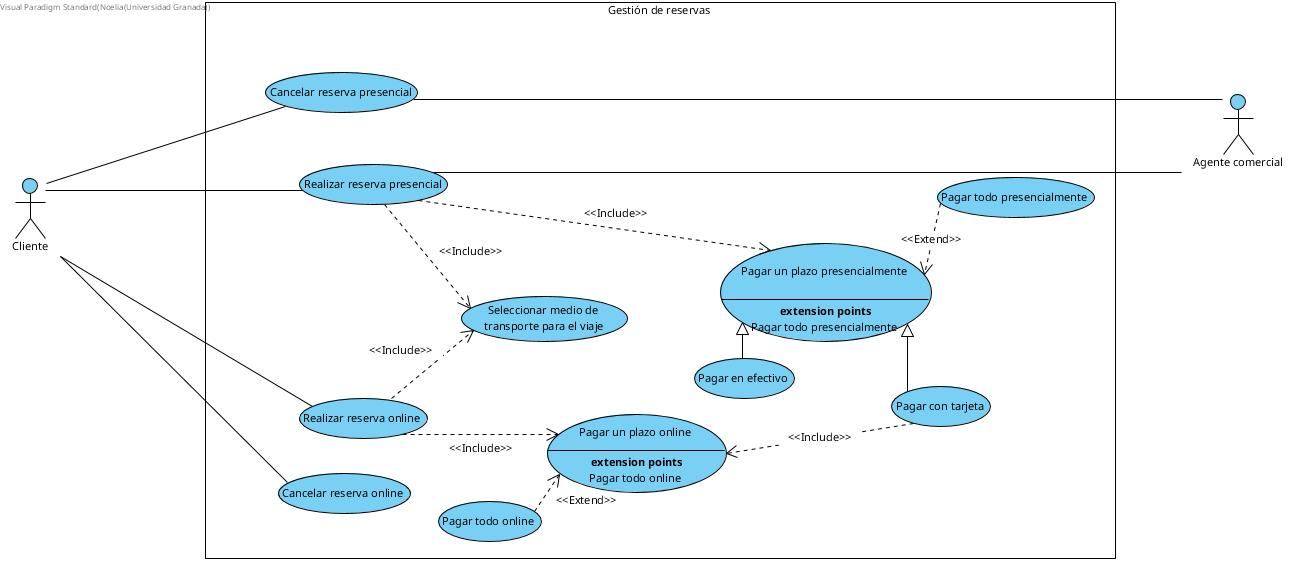
\includegraphics[totalheight=7cm]{Gestion_reservas}
		\caption{Paquete de gestión de reservas}
		\label{fig:gestion_reservas}
	\end{figure}

	\begin{figure}[H]
		\centering
		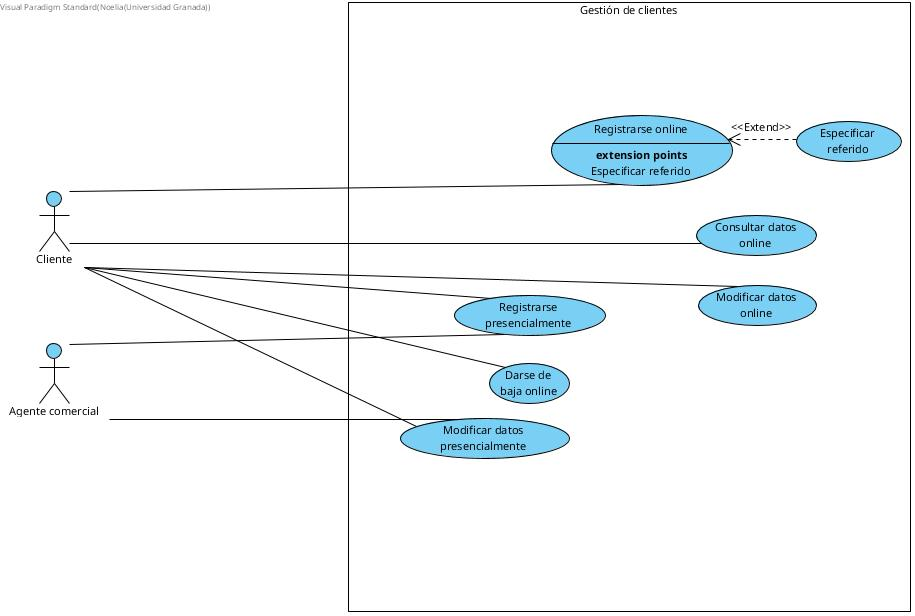
\includegraphics[totalheight=7cm]{Gestion_clientes}
		\caption{Paquete de gestión de clientes}
		\label{fig:gestion_clientes}
	\end{figure}

	\begin{figure}[H]
		\centering
		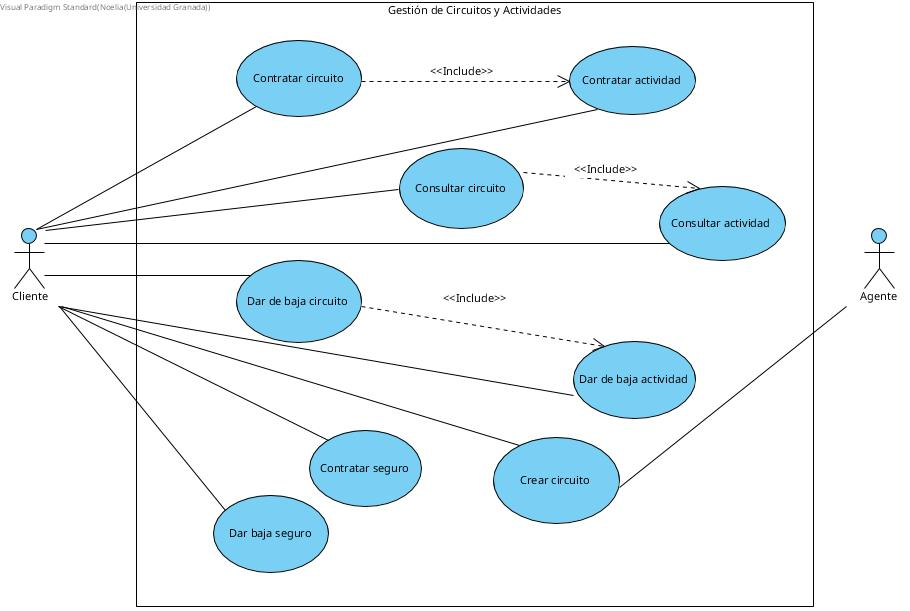
\includegraphics[totalheight=7cm]{Gestion_de_Circuitos_y_Actividades}
		\caption{Paquete de gestión de circuitos y actividades}
		\label{fig:gestion_circuitos y actividades}
	\end{figure}

	\begin{figure}[H]
		\centering
		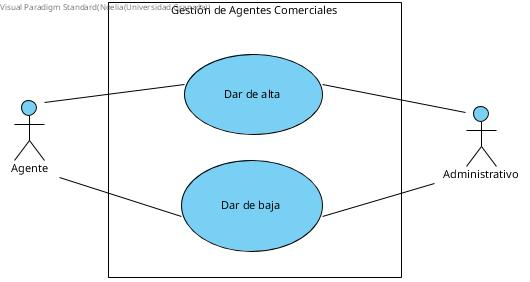
\includegraphics[totalheight=5cm]{GestionDeAgentes}
		\caption{Paquete de gestión de agentes}
		\label{fig:gestion_agentes}
	\end{figure}

	\begin{figure}[H]
		\centering
		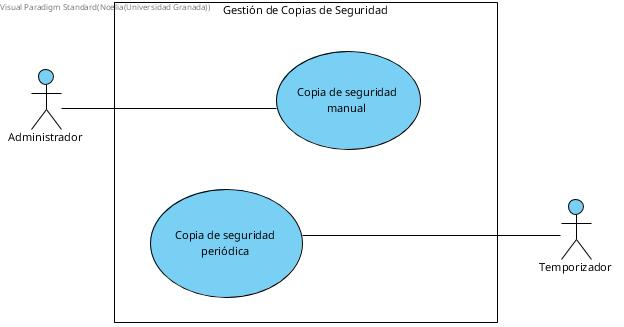
\includegraphics[totalheight=5cm]{GestionDeCopiasDeSeguridad}
		\caption{Paquete de gestión de copias de seguridad}
		\label{fig:gestion_copias_seguridad}
	\end{figure}

	\begin{figure}[H]
		\centering
		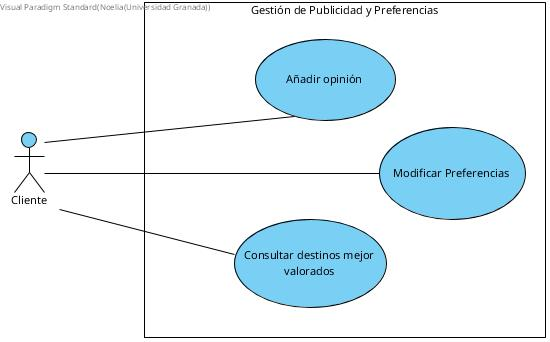
\includegraphics[totalheight=5cm]{GestionDePublicidadYPreferencias}
		\caption{Paquete de gestión de publicidad y preferencias}
		\label{fig:gestion_publicidad_preferencias}
	\end{figure}

	\section{Plantillas de actores}
	\begin{figure}[H]
		\centering
		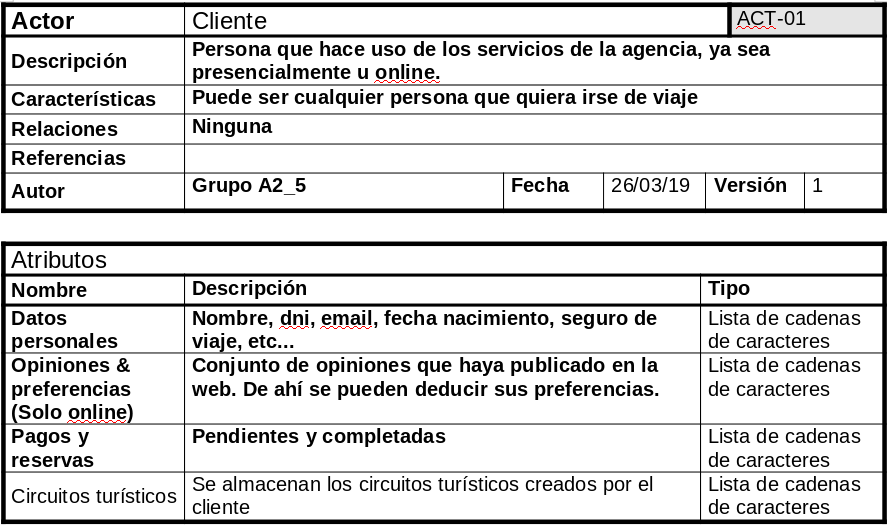
\includegraphics[totalheight=7.5cm]{act-1}
		\caption{ACT-01: Cliente}
		\label{fig:act-1}
	\end{figure}
	
	\begin{figure}[H]
		\centering
		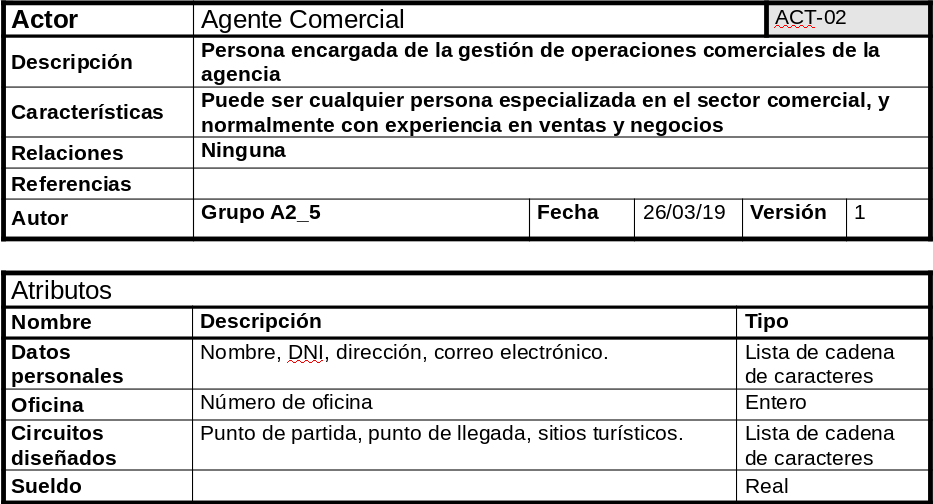
\includegraphics[totalheight=7cm]{act-2}
		\caption{ACT-02: Agente Comercial}
		\label{fig:act-2}
	\end{figure}

	\begin{figure}[H]
		\centering
		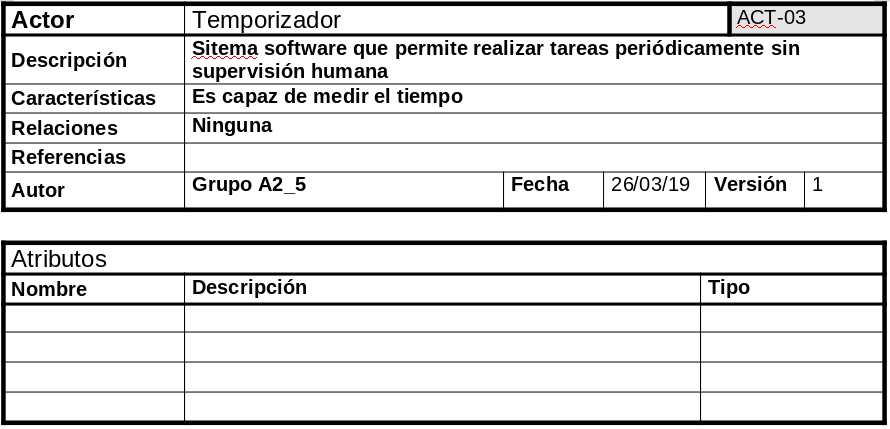
\includegraphics[totalheight=6.5cm]{act-3}
		\caption{ACT-03: Temporizador}
		\label{fig:act-3}
	\end{figure}

	\begin{figure}[H]
		\centering
		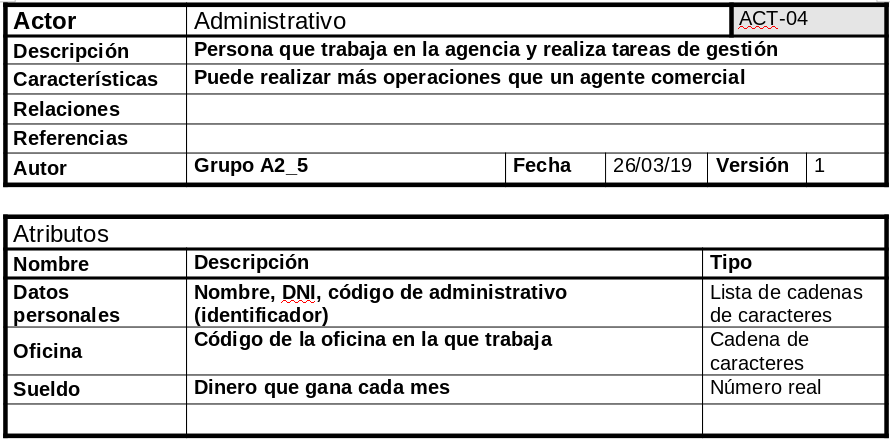
\includegraphics[totalheight=7cm]{act-4}
		\caption{ACT-04: Administrativo}
		\label{fig:act-4}
	\end{figure}

	\section{Plantillas de casos de uso}
	\begin{figure}[H]
		\centering
		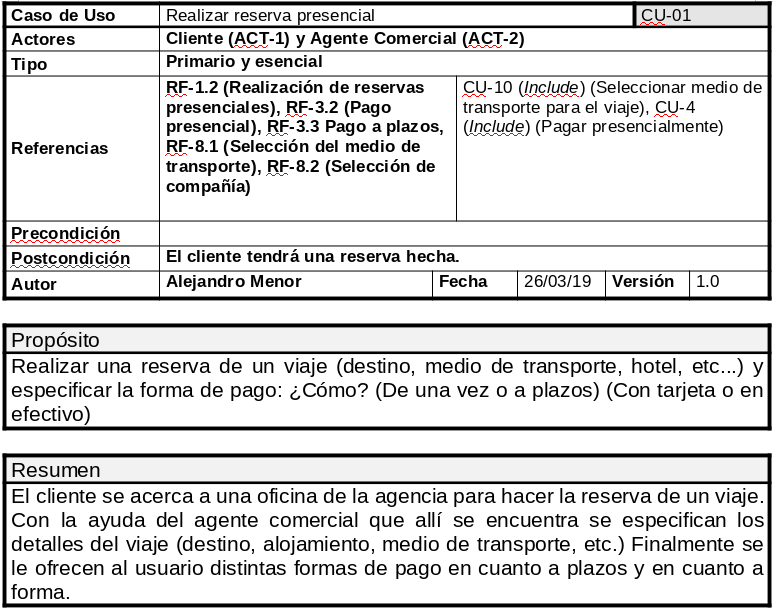
\includegraphics[totalheight=10cm]{cu-01}
		\caption{CU-01}
		\label{fig:cu-01}
	\end{figure}
	\begin{figure}[H]
		\centering
		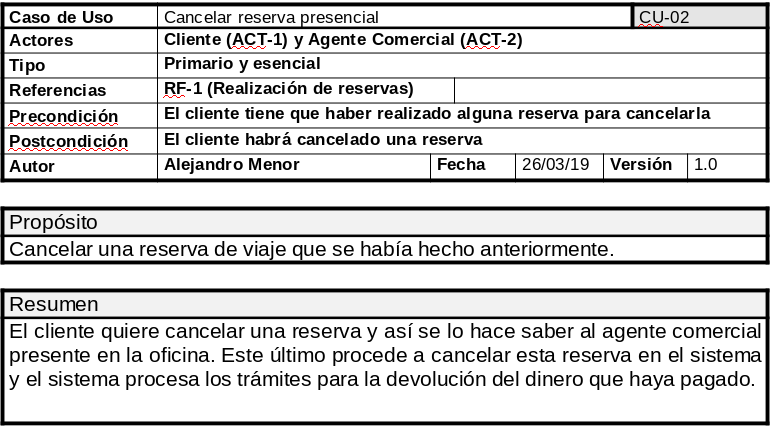
\includegraphics[totalheight=7cm]{cu-02}
		\caption{CU-02}
		\label{fig:cu-02}
	\end{figure}

	\begin{figure}[H]
		\centering
		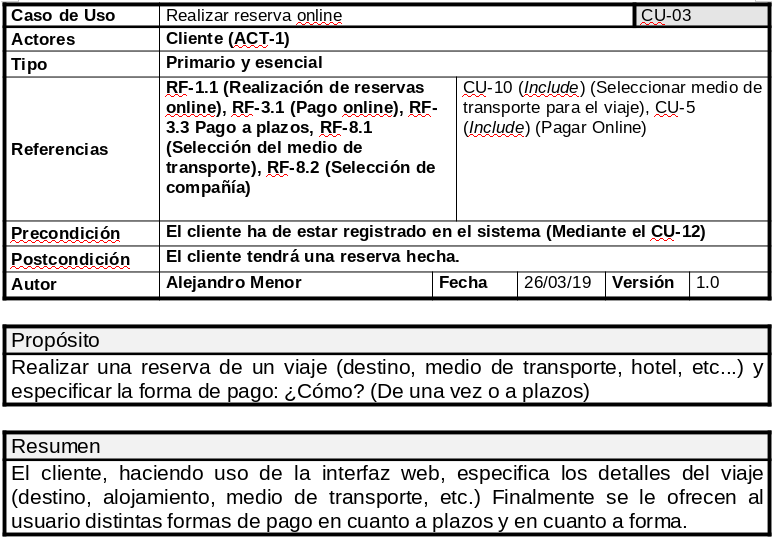
\includegraphics[totalheight=9cm]{cu-03}
		\caption{CU-03}
		\label{fig:cu-03}
	\end{figure}

	\begin{figure}[H]
		\centering
		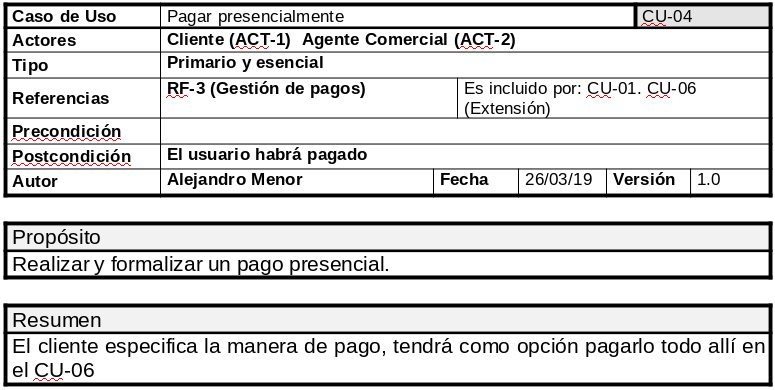
\includegraphics[totalheight=7cm]{cu-04}
		\caption{CU-04}
		\label{fig:cu-04}
	\end{figure}

	\begin{figure}[H]
		\centering
		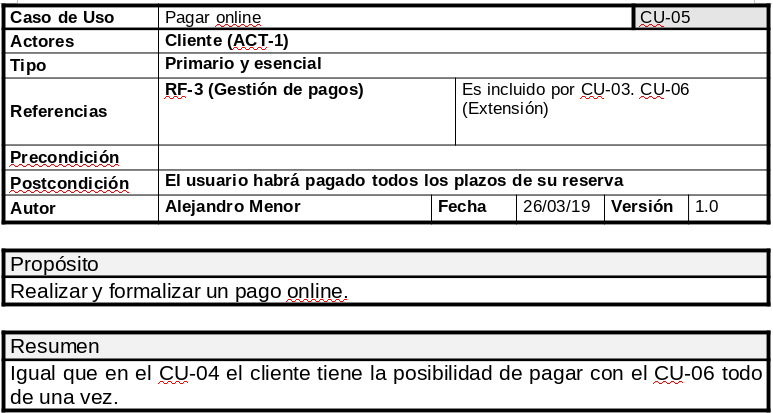
\includegraphics[totalheight=7.5cm]{cu-05}
		\caption{CU-05}
		\label{fig:cu-05}
	\end{figure}

	\begin{figure}[H]
		\centering
		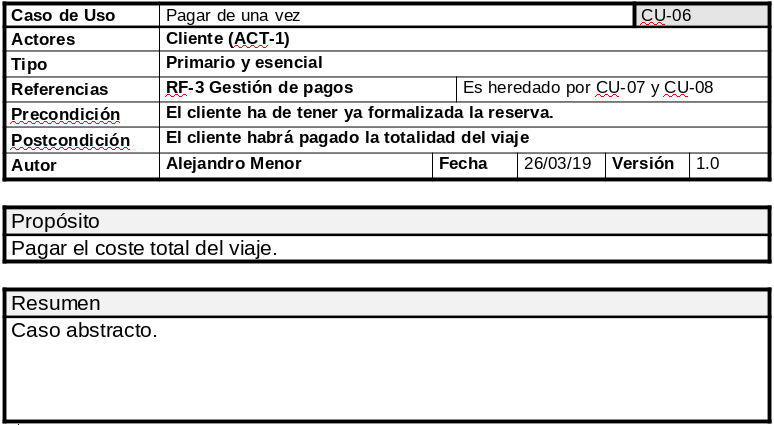
\includegraphics[totalheight=7.5cm]{cu-06}
		\caption{CU-06}
		\label{fig:cu-06}
	\end{figure}

	\begin{figure}[H]
		\centering
		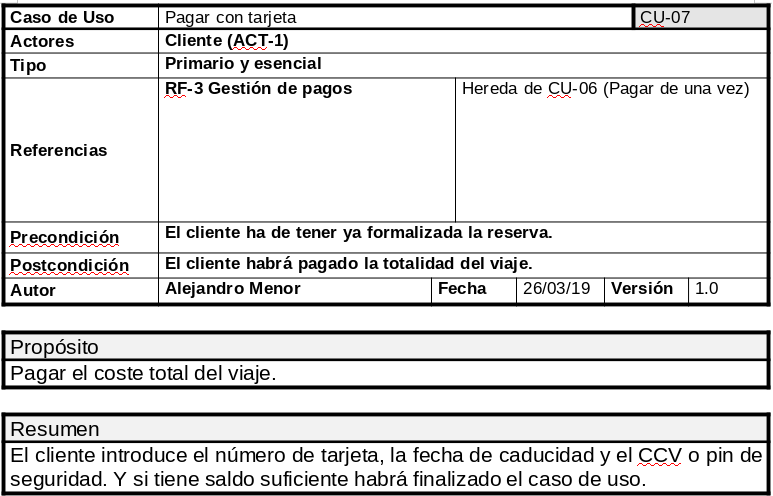
\includegraphics[totalheight=8.5cm]{cu-07}
		\caption{CU-07}
		\label{fig:cu-07}
	\end{figure}

	\begin{figure}[H]
		\centering
		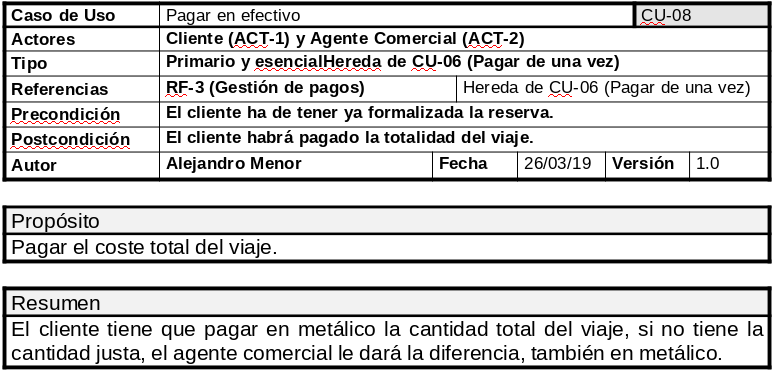
\includegraphics[totalheight=7cm]{cu-08}
		\caption{CU-08}
		\label{fig:cu-08}
	\end{figure}

	\begin{figure}[H]
		\centering
		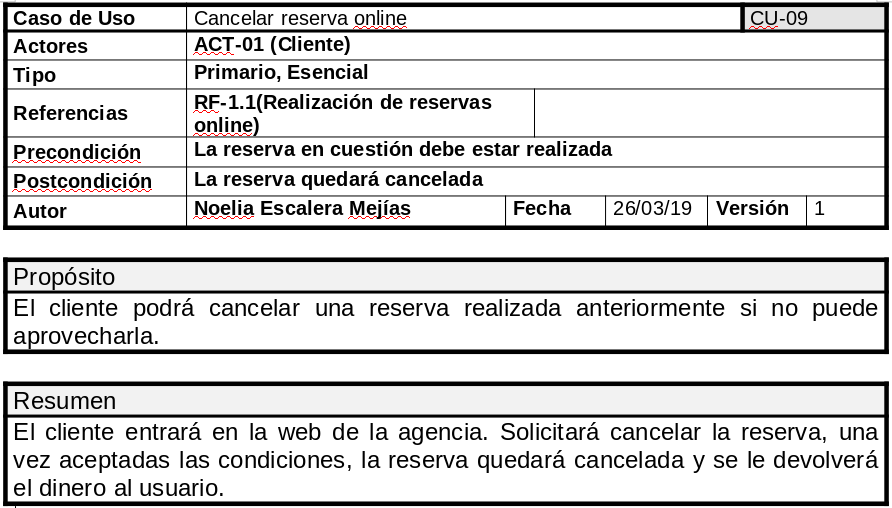
\includegraphics[totalheight=8.5cm]{cu-09}
		\caption{CU-09}
		\label{fig:cu-09}
	\end{figure}

	\begin{figure}[H]
		\centering
		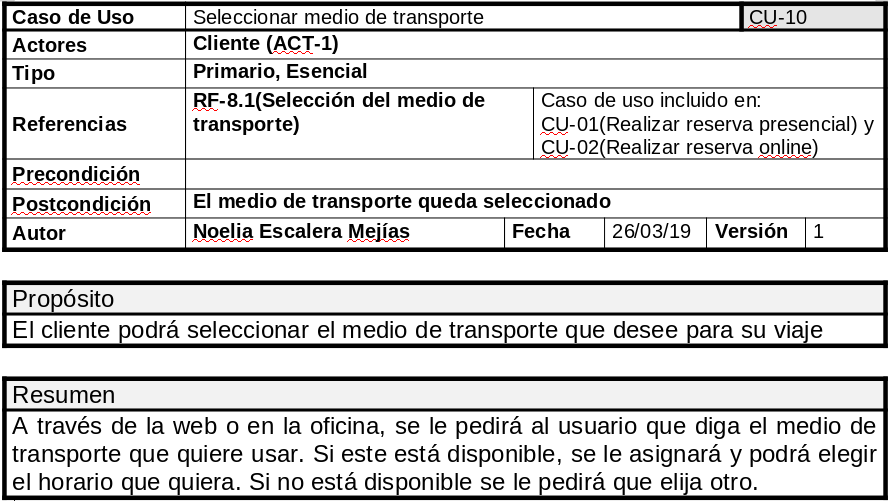
\includegraphics[totalheight=8.5cm]{cu-10}
		\caption{CU-10}
		\label{fig:cu-10}
	\end{figure}

	\begin{figure}[H]
		\centering
		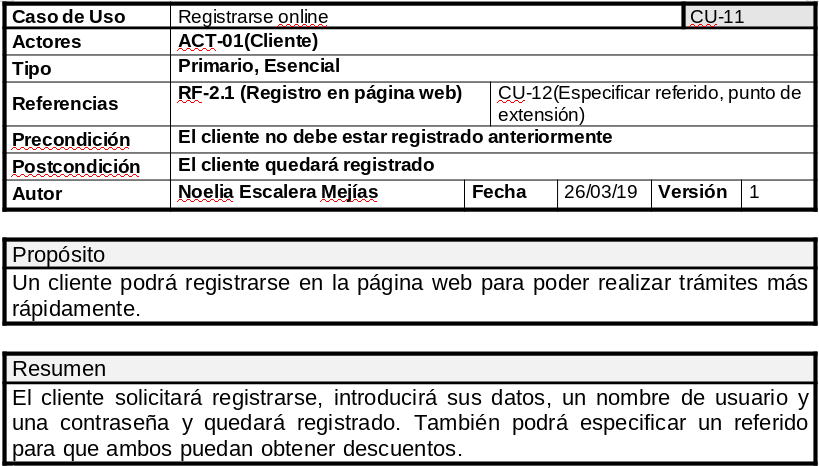
\includegraphics[totalheight=8cm]{cu-11}
		\caption{CU-11}
		\label{fig:cu-11}
	\end{figure}

	\begin{figure}[H]
		\centering
		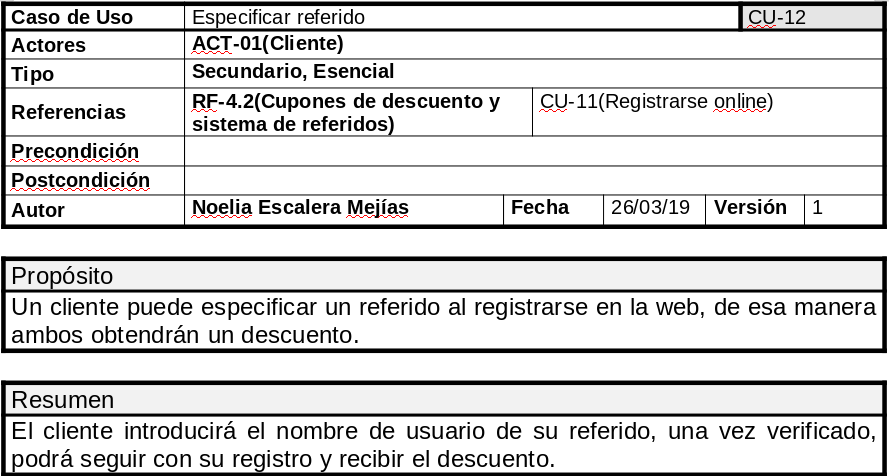
\includegraphics[totalheight=8cm]{cu-12}
		\caption{CU-12}
		\label{fig:cu-12}
	\end{figure}

	\begin{figure}[H]
		\centering
		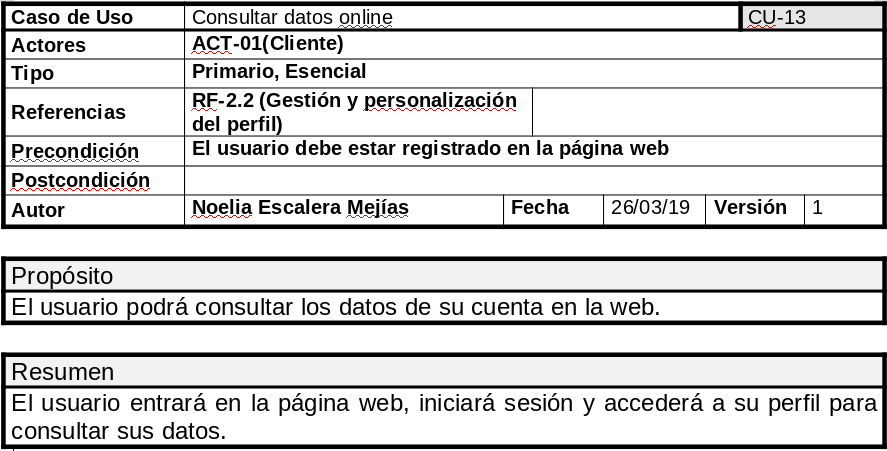
\includegraphics[totalheight=8cm]{cu-13}
		\caption{CU-13}
		\label{fig:cu-13}
	\end{figure}

	\begin{figure}[H]
		\centering
		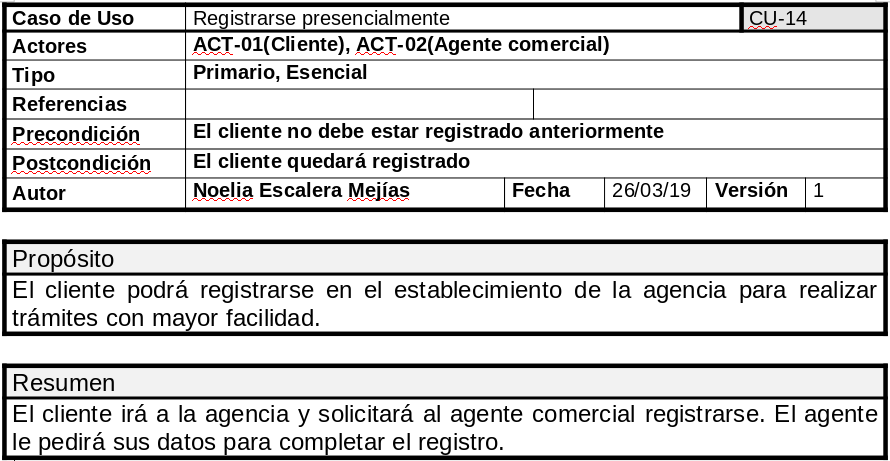
\includegraphics[totalheight=8cm]{cu-14}
		\caption{CU-14}
		\label{fig:cu-14}
	\end{figure}

	\begin{figure}[H]
		\centering
		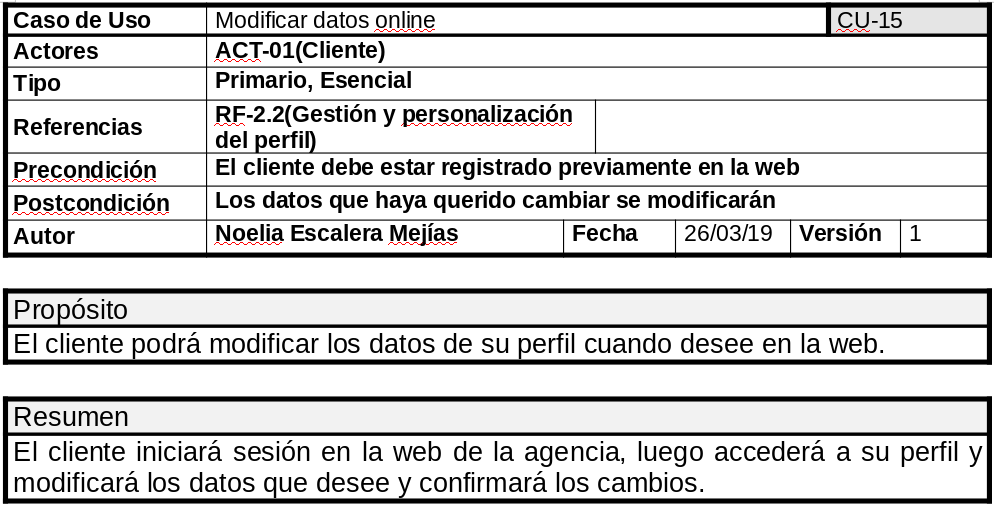
\includegraphics[totalheight=8cm]{cu-15}
		\caption{CU-15}
		\label{fig:cu-15}
	\end{figure}

	\begin{figure}[H]
		\centering
		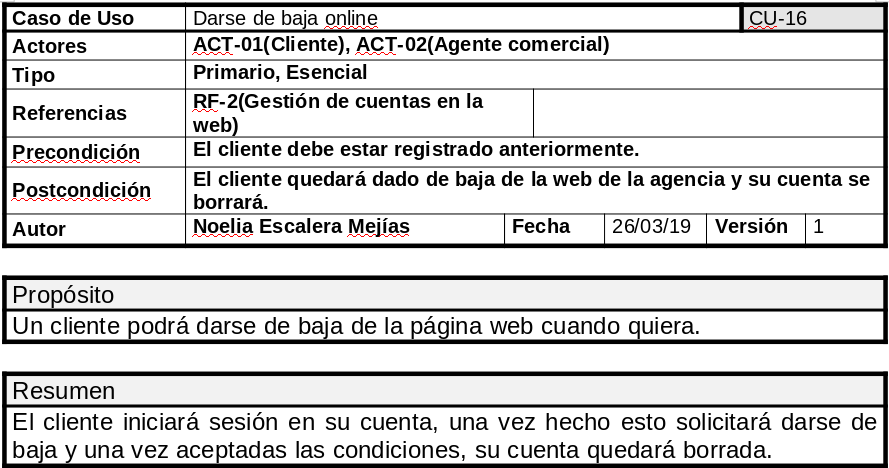
\includegraphics[totalheight=8cm]{cu-16}
		\caption{CU-16}
		\label{fig:cu-16}
	\end{figure}

	\begin{figure}[H]
		\centering
		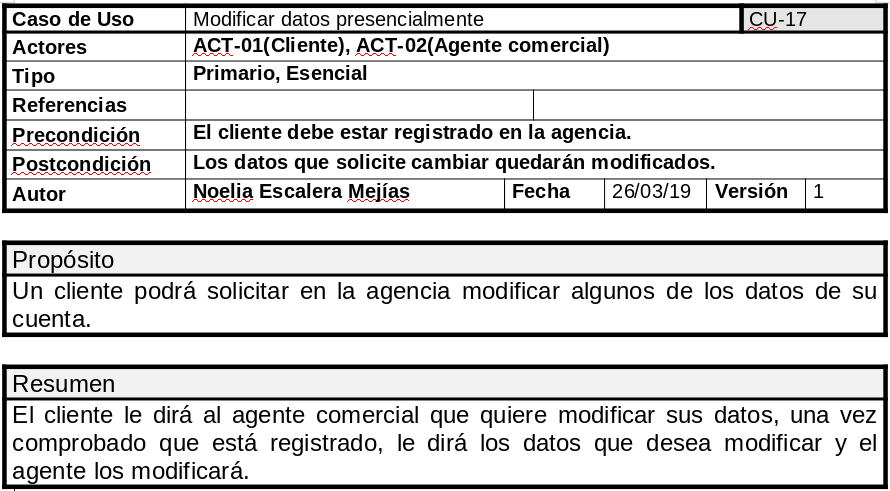
\includegraphics[totalheight=8cm]{cu-17}
		\caption{CU-17}
		\label{fig:cu-17}
	\end{figure}

	\begin{figure}[H]
		\centering
		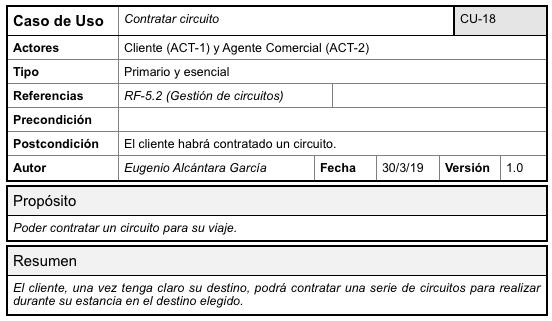
\includegraphics[totalheight=8cm]{CU-18}
		\caption{CU-18}
		\label{fig:cu-18}
	\end{figure}

	\begin{figure}[H]
		\centering
		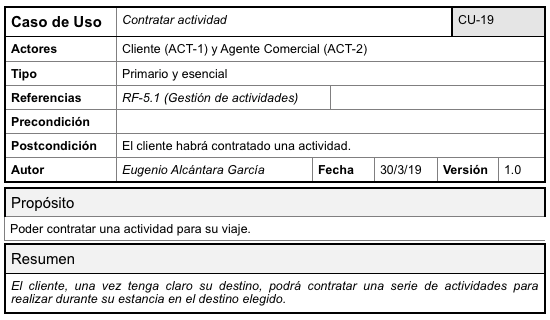
\includegraphics[totalheight=8cm]{CU-19}
		\caption{CU-19}
		\label{fig:cu-19}
	\end{figure}

	\begin{figure}[H]
		\centering
		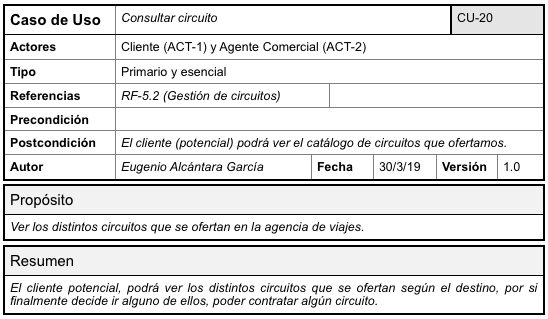
\includegraphics[totalheight=8cm]{CU-20}
		\caption{CU-20}
		\label{fig:cu-20}
	\end{figure}

	\begin{figure}[H]
		\centering
		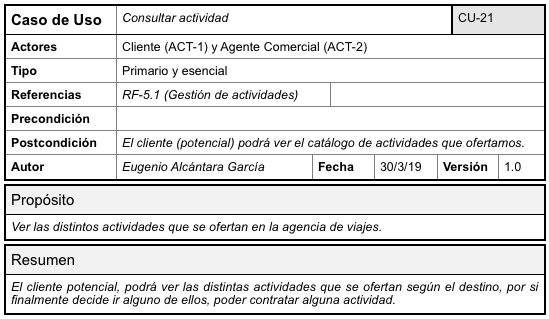
\includegraphics[totalheight=8cm]{CU-21}
		\caption{CU-21}
		\label{fig:cu-21}
	\end{figure}

	\begin{figure}[H]
		\centering
		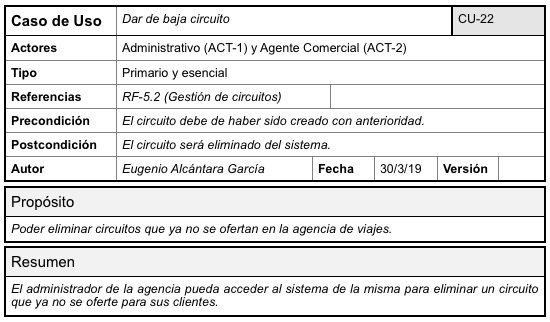
\includegraphics[totalheight=8cm]{CU-22}
		\caption{CU-22}
		\label{fig:cu-22}
	\end{figure}

	\begin{figure}[H]
		\centering
		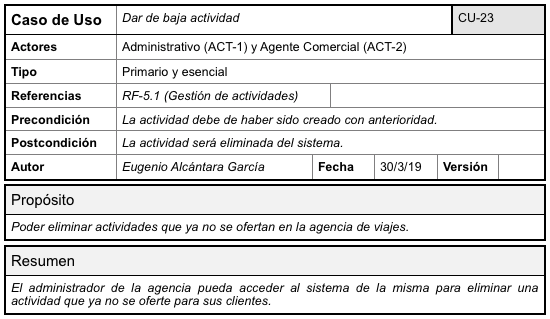
\includegraphics[totalheight=8cm]{CU-23}
		\caption{CU-23}
		\label{fig:cu-23}
	\end{figure}

	\begin{figure}[H]
		\centering
		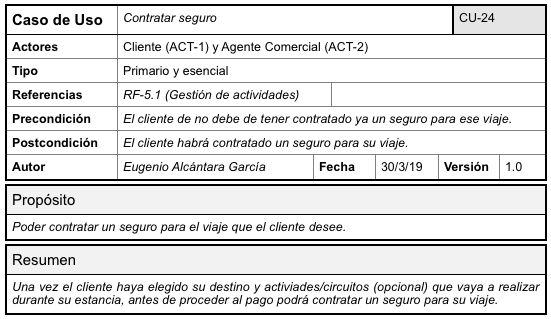
\includegraphics[totalheight=8cm]{CU-24}
		\caption{CU-24}
		\label{fig:cu-24}
	\end{figure}

	\begin{figure}[H]
		\centering
		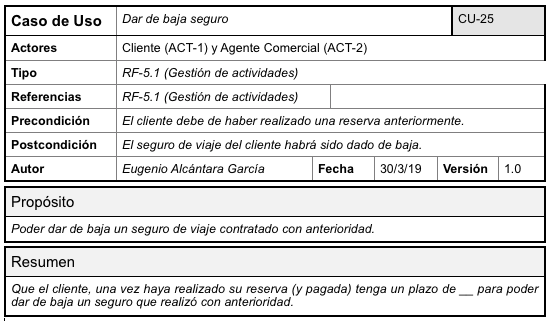
\includegraphics[totalheight=8cm]{CU-25}
		\caption{CU-25}
		\label{fig:cu-25}
	\end{figure}

	\begin{figure}[H]
		\centering
		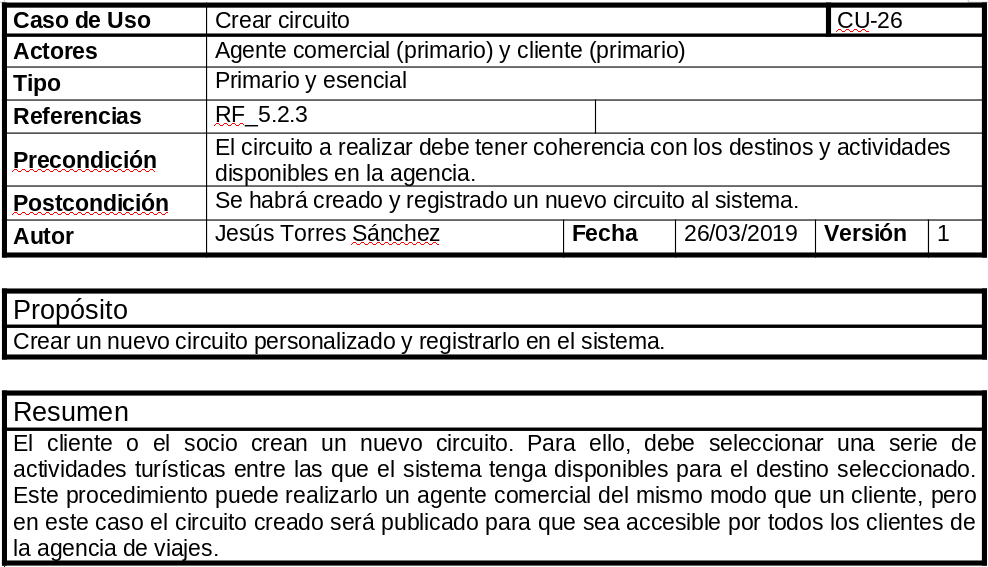
\includegraphics[totalheight=8cm]{cu-26}
		\caption{CU-26}
		\label{fig:cu-26}
	\end{figure}

	\begin{figure}[H]
		\centering
		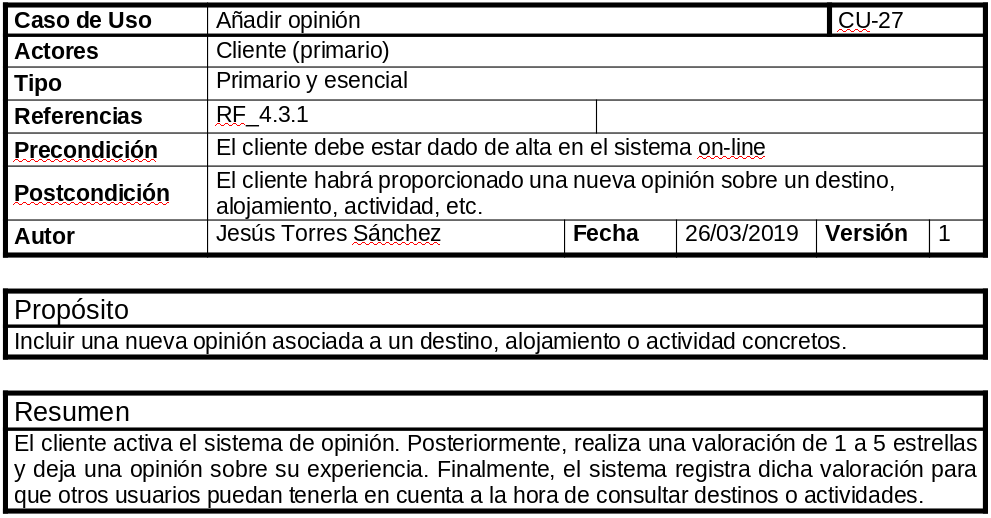
\includegraphics[totalheight=8cm]{cu-27}
		\caption{CU-27}
		\label{fig:cu-27}
	\end{figure}

	\begin{figure}[H]
		\centering
		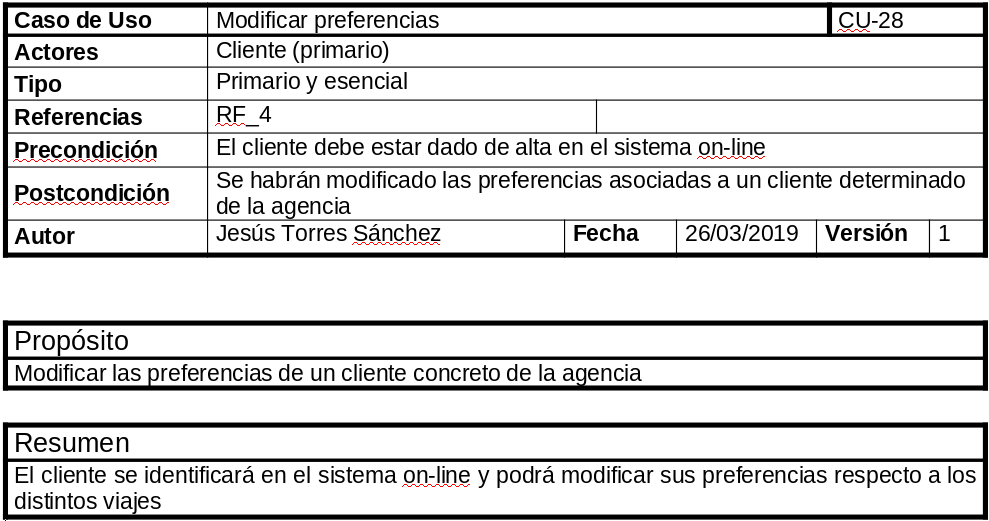
\includegraphics[totalheight=8cm]{cu-28}
		\caption{CU-28}
		\label{fig:cu-28}
	\end{figure}
	
	\begin{figure}[H]
		\centering
		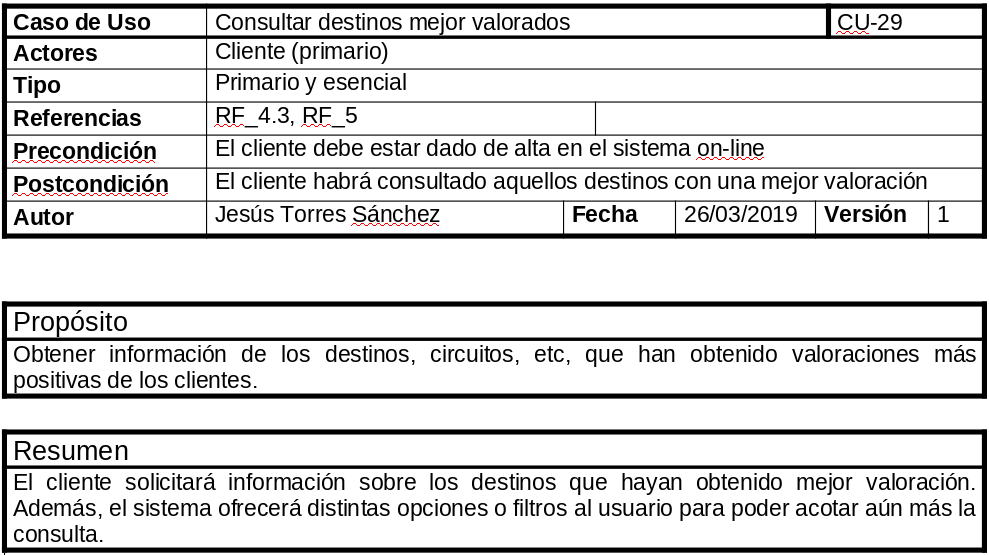
\includegraphics[totalheight=8cm]{cu-29}
		\caption{CU-29}
		\label{fig:cu-29}
	\end{figure}

	\begin{figure}[H]
		\centering
		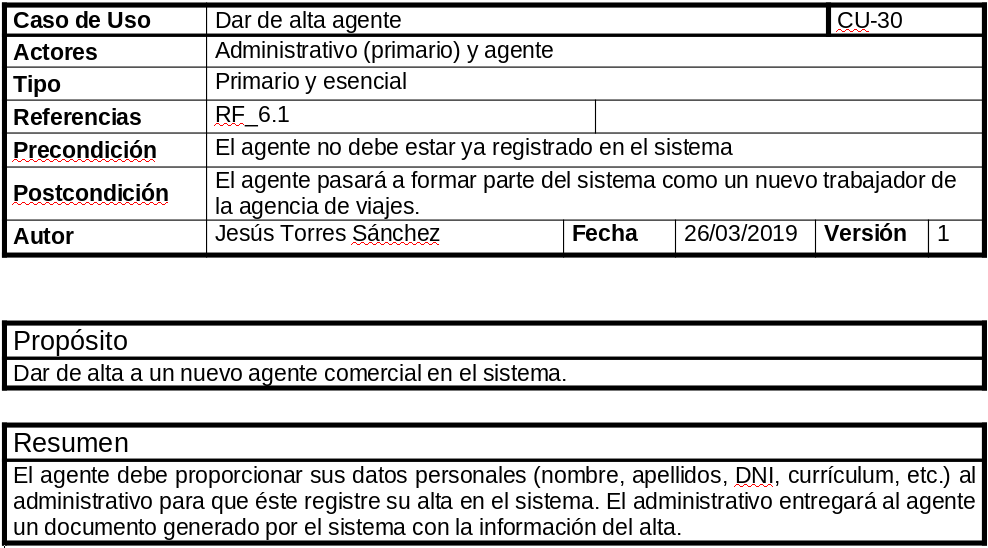
\includegraphics[totalheight=8cm]{cu-30}
		\caption{CU-30}
		\label{fig:cu-30}
	\end{figure}

	\begin{figure}[H]
		\centering
		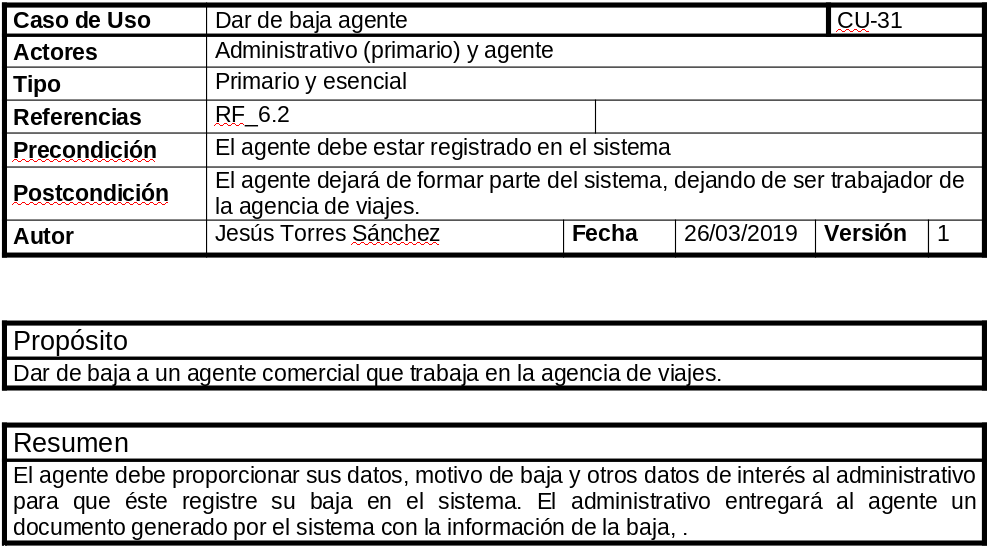
\includegraphics[totalheight=8cm]{cu-31}
		\caption{CU-31}
		\label{fig:cu-31}
	\end{figure}
		
	\begin{figure}[H]
		\centering
		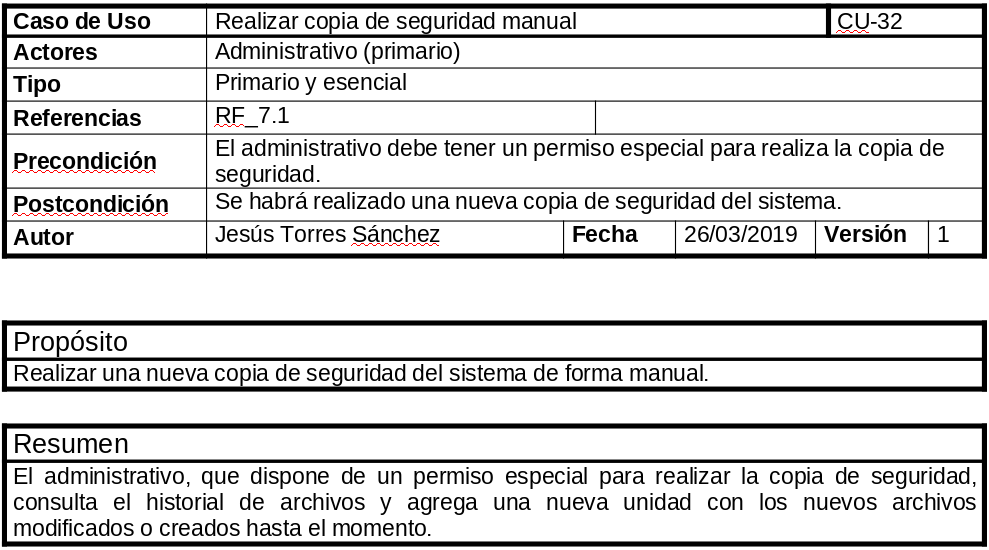
\includegraphics[totalheight=8cm]{cu-32}
		\caption{CU-32}
		\label{fig:cu-32}
	\end{figure}

	\begin{figure}[H]
		\centering
		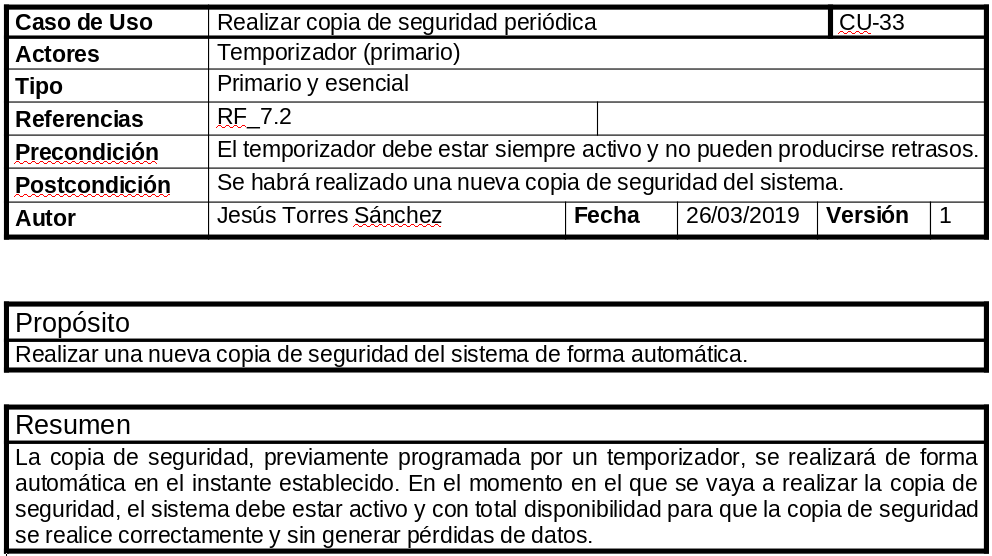
\includegraphics[totalheight=8cm]{cu-33}
		\caption{CU-33}
		\label{fig:cu-33}
	\end{figure}

	\section{Diagrama de paquetes}
	
	\begin{figure}[H]
		\centering
		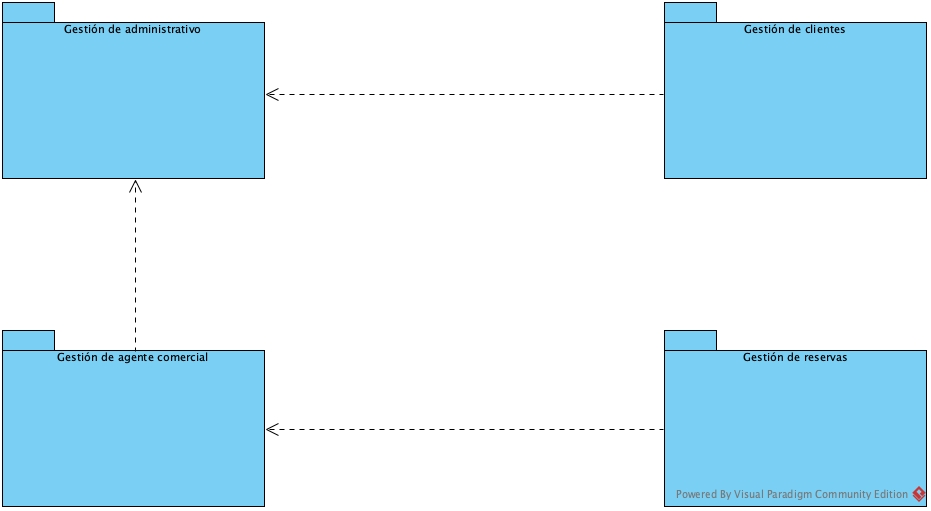
\includegraphics[totalheight=8cm]{diagrama_de_paquetes}
		\caption{Diagrama de paquetes}
		\label{fig:paquetes}
	\end{figure}
	
\end{document}